%%% COMPONENTI STRUTTURA
\section{Componenti Angular}
I componenti rappresentano l'elemento base di un'applicazione Angular e sono composti da 3 elementi principali:
\begin{itemize}
    \item Una classe Typescript che ne implementa il comportamento e le proprietà 
    \item Un template HTML che ne definisce la vista renderizzata all'interno del DOM 
    \item Un file css che ne definisce lo stile
\end{itemize}
Il comportamento dei componenti viene fornito da una direttiva Component che fornisce i metadati necessari alla creazione gestione e eliminazione del componente tra cui:
\begin{itemize}
    \item Il CSS selector
    \item Il template del componente
    \item Il foglio di stile 
    \item I provider degli eventuali servizi di cui il componente potrà usufruire
\end{itemize}
In particolare è proprio il @Component decorator che identifica la classe Typescript come componente alla libreria angular, il quale senza non viene riconosciuto come tale.
\newline
Una parte fondamentale di ogni componente è il CSS selector che è il nome con cui viene riconosciuto dalla libreria e indica di renderizzare il componente ogni qualvolta viene trovato il corrispettivo tag.
\newline
\subsection{Angular template}
Il template definisce ciò che viene renderizzato nel DOM all'istanziazione,
al suo interno è possibile sfruttare il data binding dei componenti  per referenziare le proprietà definite nella classe typescript e sfruttare le direttive Angular per rendere dinamica la costruzione del DOM. 
\newline
\newline
\begin{figure}[H]
    \centering
    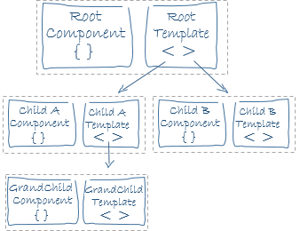
\includegraphics[scale=1]{resources/component-tree.png}
    \cite{angular-doc}
    \caption{struttura albero dei componenti}
\end{figure}

Il template di un componente e la sua classe typescript formano una view, la quale può includere altre view al suo interno in una struttura gerarchica ad albero.
\newline
Il template di un componente angular è scritto in codice HTML esteso dalla sintassi Angular per il template, la quale si occupa di alterare il DOM a seconda della logica applicativa e della variazione dei dati.
Come già anticipato, all'interno del template è possibile sfruttare:
\begin{itemize}
    \item Direttive per applicare logica al rendering del component (ngFor)
    \item Pipe per trasformare i dati prima di mostrarli a schermo 
    \item Data binding tra proprietà della classe e template
\end{itemize}
Le direttive sono classi typescript contenenti il decorator @directive che consentono di rendere il template dei componenti dinamico e si suddividono in due tipologie:
\begin{itemize}
    \item Direttive strutturali
    \item Direttive attributo
\end{itemize}
Le direttive strutturali alterano il DOM aggiungendo rimuovendo o modificando elementi come le direttive ngFor e ngIf,
mentre le direttive attributo alterano il DOM modificando il valore di singoli attributi.
\newline
\newline
Le pipe sono strumenti attraverso i quali è possibile manipolare i dati da mostrare nel DOM tramite particolari sequenze di istruzioni come per esempio la formattazione di dati nel formato locale dell'utente oppure la formattazione di valute.
\newline
\newline
Una delle operazioni più tediose e inclini alla generazione di errori nelle interfacce web è la necessità di collegare i dati mostrati all'interno dell'interfaccia con ciò che viene manipolato dalla logica applicativa. Tramite il data binding la libreria Angular automatizza questo processo come mostrato nell'immagine sottostante
\newline
\newline
\begin{figure}[H]
    \centering
    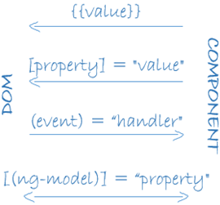
\includegraphics[scale=1]{resources/databinding.png}
    \cite{angular-doc}
    \caption{Modalità di funzionamento data binding}
\end{figure}
nell'immagine viene mostrata la possibilità di implementazione del data binding in 3 possibili modalità:
\begin{itemize}
    \item Monodirezionale dal component al dom
    \item Monodirezionale dal dom al component
    \item Bidirezionale
\end{itemize}
In questo modo viene automatizzata una procedura molto onerosa e che molto spesso rende illeggibili le interfacce di molte applicazioni web